\documentclass[10.5pt,a4paper]{article}
\usepackage[a4paper,left=2.6cm,right=2.6cm,top=2.6cm,bottom=2.5cm]{geometry}
\usepackage{fontspec}
\usepackage{xeCJK}
\setCJKmainfont{AR PL SungtiL GB}[AutoFakeBold=2.5]
\setCJKsansfont{AR PL SungtiL GB}[AutoFakeBold=2.5]
\usepackage{xcolor,graphicx,booktabs,array,amsmath,titlesec,enumitem,caption,float,indentfirst}
\titleformat{\section}{\bfseries\large}{\thesection}{.7em}{}
\titleformat{\subsection}{\bfseries\normalsize}{\thesubsection}{.6em}{}
\titlespacing*{\section}{0pt}{1.4em}{.6em}\titlespacing*{\subsection}{0pt}{1em}{.4em}
\pagestyle{plain}
\renewcommand{\figurename}{图}\renewcommand{\tablename}{表}
\captionsetup{font=small,labelfont=bf,labelsep=quad,skip=4pt}
\setlist[itemize]{leftmargin=1.6em,itemsep=1pt,topsep=2pt,parsep=0pt}
\setlist[enumerate]{leftmargin=1.8em,itemsep=1pt,topsep=2pt,parsep=0pt}
\setlength{\parindent}{2em}\setlength{\parskip}{0pt}\linespread{1.25}
\renewcommand{\arraystretch}{1.15}
\newcommand{\bv}[1]{\textbf{#1}}
\begin{document}

\begin{center}{\LARGE\bfseries Rayleigh--B\'enard 稀疏观测同化：\\滞后（lag）初始化 EnKF 对比\par}\vspace{.4em}{\small 基于已保存的实验结果；初始化对 EnKF 含有真值信息，见第 5 节}\end{center}

\section{目的与假设}
前期主实验中 EnKF 的初始集合以 A1 第 0 帧分析为中心加扰动。该集合起点离散度小、且借用了 A1 的结果，与 EnKF 的常规用法不同。本文用另一种构造：\textbf{取同一条轨迹的第 0--19 帧，各自用求解器积分到第 40 帧，作为 20 个成员；从第 40 帧开始同化，评价第 40--99 帧（共 60 帧）。}假设是：在这样的集合下，观测间隔 $K$ 增大时 A1 相对 EnKF 的优势会发生变化。若 A1 在所有 $K$ 下仍占优，则此前的结论稳固；若在大 $K$ 下 EnKF 更优，则此前``K 大时 A1 略优''的结论依赖于初始化。

\section{设置}
\begin{itemize}
\item 状态、先验、观测噪声（0.1）、观测比例（1\%）、预报求解器（Ra$=5\times10^4$，真值 $10^5$）、A1 的全部参数均与主实验相同，未为本实验重调。
\item \textbf{EnKF 初始集合：}真值第 $i$ 帧（$i=0,\dots,19$）经求解器积分 $40-i$ 帧至第 40 帧，得到 20 个成员；不额外加噪声；EnKF 在第 40 帧也做同化；20 成员、乘性膨胀、不用局地化。
\item \textbf{A1 与纯预报：}从第 40 帧冷启动。第 40 帧无背景、只用该帧观测；之后每 $K$ 帧同化一次。纯预报为第 40 帧同化后不再同化。
\item 测试 20 个轨迹，种子 42/43/44；观测位置、噪声、采样噪声由种子决定，三种方法在同一轨迹、同一种子下看到相同的观测。
\item EnKF 膨胀在 5 个验证轨迹（种子 42）上选，见下表；测试轨迹只用于最终评估。
\end{itemize}
\begin{table}[H]\centering\small\caption{验证轨迹上各膨胀系数的 EnKF 平均 RMSE（第 40--99 帧）。}
\begin{tabular}{cp{10.5cm}}\toprule
$K$ & 膨胀系数: RMSE\\\midrule
1 & 1.0: 0.0290，1.1: 0.0229，1.2: 0.0235，1.4: 0.0281 \\
5 & 1.0: 0.0319，1.1: 0.0295，1.2: 0.0272，1.4: 0.0253，1.6: 0.0254，2.0: 0.0271 \\
10 & 1.0: 0.0328，1.1: 0.0319，1.2: 0.0307，1.4: 0.0284，1.6: 0.0271，2.0: 0.0266 \\
20 & 1.0: 0.0334，1.1: 0.0330，1.2: 0.0326，1.4: 0.0315，1.6: 0.0302，2.0: 0.0282 \\
\bottomrule\end{tabular}\end{table}
$K=10,20$ 的最优膨胀落在扫描区间的上边界（2.0），未继续扩大，因此这两个 $K$ 下的 EnKF 可能仍有改善空间。

\section{结果}
\begin{table}[H]\centering\small\caption{测试集 20 个轨迹的未观测点 RMSE（第 40--99 帧，种子 42 / 43 / 44）。``降低''为 A1 相对 EnKF 的降低，负值表示 A1 更差；``A1 更优''为 20 个轨迹中 A1 误差更小的个数。}
\resizebox{\linewidth}{!}{\begin{tabular}{cccccccc}\toprule
$K$ & 膨胀 & A1 & EnKF (lag) & 纯预报 & 降低 & A1 更优\\\midrule
1 & 1.1 & 0.0156 / 0.0164 / 0.0155 & 0.0230 / 0.0237 / 0.0228 & 0.0407 / 0.0454 / 0.0375 & +32\% / +31\% / +32\% & 20 / 20 / 20 \\
5 & 1.4 & 0.0223 / 0.0232 / 0.0213 & 0.0252 / 0.0256 / 0.0253 & 0.0407 / 0.0454 / 0.0375 & +11\% / +9\% / +16\% & 16 / 15 / 19 \\
10 & 2.0 & 0.0289 / 0.0318 / 0.0283 & 0.0260 / 0.0269 / 0.0256 & 0.0407 / 0.0454 / 0.0375 & -11\% / -18\% / -10\% & 5 / 5 / 6 \\
20 & 2.0 & 0.0348 / 0.0392 / 0.0329 & 0.0292 / 0.0295 / 0.0288 & 0.0407 / 0.0454 / 0.0375 & -19\% / -33\% / -14\% & 3 / 1 / 5 \\
\bottomrule\end{tabular}}\end{table}
\begin{figure}[H]\centering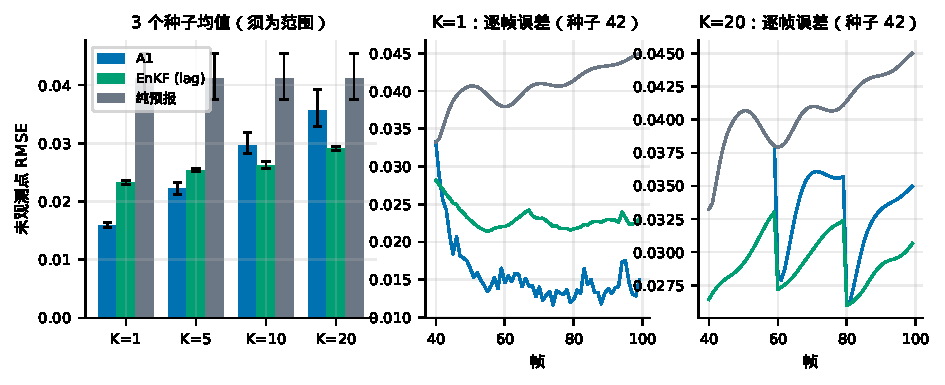
\includegraphics[width=\linewidth]{report_fig_lag/main.pdf}\caption{左：各观测间隔下的误差；中、右：$K=1$、$K=20$ 的逐帧误差。}\end{figure}
\begin{figure}[H]\centering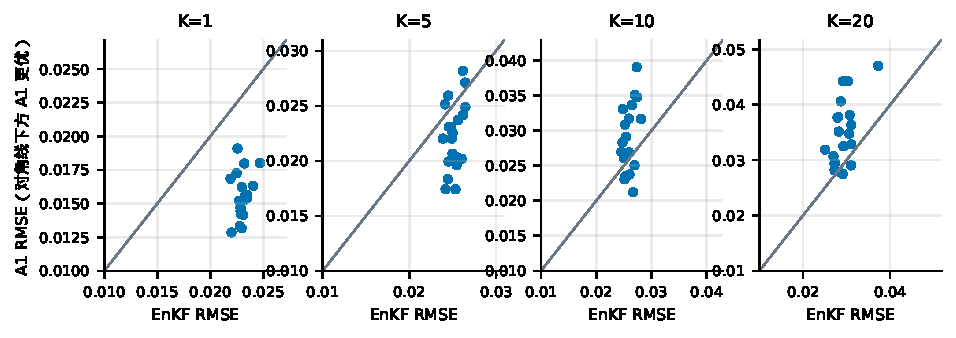
\includegraphics[width=\linewidth]{report_fig_lag/cases.pdf}\caption{逐轨迹配对比较（种子 42）。}\end{figure}
$K=1,5$ 时 A1 更优（误差分别低 31--32\% 与 9--16\%）；$K=10,20$ 时 EnKF 更优（A1 误差分别高 10--18\% 与 14--33\%，三个种子的范围）。逐轨迹看，大 $K$ 下 A1 只在少数轨迹上更优。

\subsection{与主实验初始化的对照}
同样取第 40--99 帧，主实验（EnKF 以 A1 第 0 帧分析为中心加扰动、第 0 帧起连续同化；$K=20$ 用膨胀 1.4）的结果如下，3 个种子均值：
\begin{table}[H]\centering\small\caption{主实验初始化下第 40--99 帧的 RMSE。}
\begin{tabular}{cccc}\toprule
$K$ & A1 & EnKF（中心加扰动） & A1 降低\\\midrule
1 & 0.0145 & 0.0241 & +40\% \\
20 & 0.0361 & 0.0408 & +12\% \\
\bottomrule\end{tabular}\end{table}
两种初始化下 $K=1$ 时 A1 都占优；$K=20$ 时结论相反。这说明大 $K$ 下的 A1--EnKF 比较\textbf{取决于 EnKF 的初始化}，不能单独引用任一组数字作为总体结论。

\section{EnKF 初始集合的性质}
lag 集合在第 40 帧的离散度（spread）约 0.0040，集合均值对真值的误差约 0.0296，即误差约为 spread 的 7 倍，集合明显偏自信（离散度小于实际误差）；观测更新量因此偏小，实验中靠较大的膨胀系数补偿。主实验中的中心加扰动集合：spread 约 0.014、误差约 0.038（比值约 2.7）。

\section{需要如实说明的限制}
\begin{enumerate}
\item \textbf{信息泄漏：}lag 集合使用了测试轨迹真值的前 20 帧，A1 没有用到。EnKF 在 $K\ge10$ 时更优，有多少来自这部分真值信息，本文\textbf{没有做拿掉真值的对照}，不能断言是 EnKF 方法本身更好。
\item \textbf{起点不对等：}A1 在第 40 帧冷启动，没有历史。对 $K=20$ 的单种子检查显示：A1 冷启动与从第 0 帧连续同化相比，起点后前 10 帧误差高约 13\%（0.0375 对 0.0332），之后 50 帧并不更差（0.0342 对 0.0369）。这是单种子、两次运行随机数流不同的比较，差异在噪声范围内，不是严格结论。
\item \textbf{A1 的参数在 $K=1$ 下选定，}$K=5,10,20$ 及 lag 设置下没有重调；$K=10,20$ 的 EnKF 膨胀在扫描边界。两边调参预算不对等。
\item 评价窗口只有 60 帧，$K=20$ 时仅 3 次同化（第 40、60、80 帧），统计量有限，不能与 100 帧的主表直接比较。
\item 成员的积分时长不同（21--40 帧），不是同一预报时长的标准集合。
\item 3 个种子、20 个轨迹；Ra 失配只有 Ra$=5\times10^4$ 一档；模型误差较弱（纯预报约 0.041）也限制了不同方法之间的区分度。
\end{enumerate}

\section{结论}
\begin{itemize}
\item 观测密（$K=1,5$）时，A1 在两种 EnKF 初始化下都优于调优的 EnKF。
\item 观测稀疏（$K\ge10$）时，在 lag 初始化下 EnKF 更优；在中心加扰动初始化下 A1 略优。两种设置的差别包含真值信息泄漏，目前无法分离原因。
\item 下一步应补做不含真值的 EnKF 初始化（例如用独立预热的集合），并在相同起点下重调 A1 的 $K=5,10,20$ 参数，再下结论。
\end{itemize}
\end{document}
